\chapter{Results and discussion}

\section{Data exploration}
As described earlier in Chapter 3, the data for the experiments is from Twitter. It was extracted and pre-processed by \cite{preotiuc-pietro_automatically_2019} and further enhanced with the labels for complaint severity by \cite{jinModelingSeverityComplaints2021}. What follows are the key findings from the exploratory data analysis performed. Additionally, some minor differences in the distribution of the tweets across the domains are observed between the latest version of the dataset available in the public domain\footnote{\url{https://archive.org/details/complaint_severity_data}} and the distribution described in the original paper. Since the variations are minor (0.5 to 2\%), any potential impact on the model performance should be insignificant in the context of the objectives of the experiments.

\begin{figure}[htbp]
    \centering
    \captionsetup{font=small}
    \begin{subfigure}{0.49\textwidth}
        \centering
        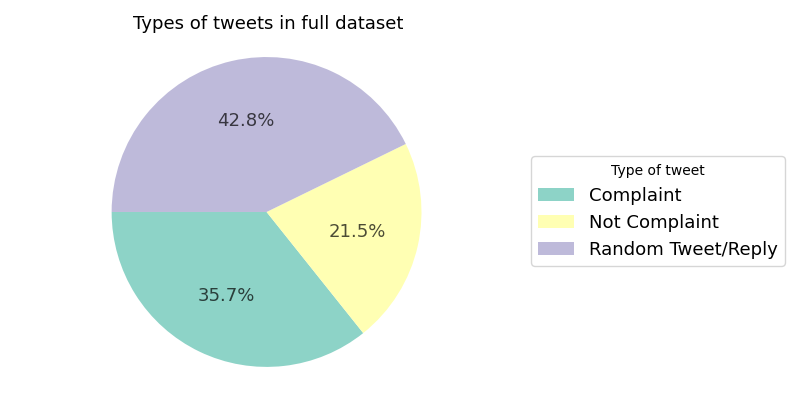
\includegraphics[width=\linewidth]{figures/compl_non_random_dist.png}
        \caption{Types of tweets}
        \label{fig: compl_non_random_dist}
    \end{subfigure}
    \hfill
    \begin{subfigure}{0.49\textwidth}
        \centering
        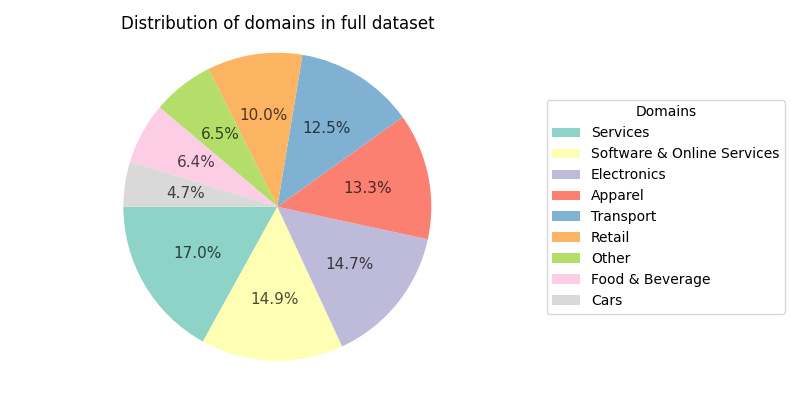
\includegraphics[width=\linewidth]{figures/domain_dist.png}
        \caption{Proportion of each domains}
        \label{fig: domain_dist}
    \end{subfigure}
    \caption{ \ref{fig: compl_non_random_dist} illustrates the distribution of tweets categorized as 'complaints' and 'not complaints', with random 'tweets / replies' shown separately. Figure \ref{fig: domain_dist}, on the other hand, presents the domain proportions within the two categories of tweets, 'complaints' and 'not complaints'.}
    \label{fig: compl_main_dist}
\end{figure}

All tweets that are complaints have \texttt{label:1} and any tweet that is not a complaint has \texttt{label:0}. From a class balance perspective, the dataset is weighted in favour of 'not complaint' tweets as can be seen in Figure \ref{fig: compl_non_random_dist}, with \texttt{label:1} at 35.7\% vs \texttt{label:0} at 64.3\%. The authors of \cite{preotiuc-pietro_automatically_2019} included several random tweets and replies to allow the model to generalise better and not be 

\section{Comparision of model performance}
**TO UPDATE**

\section{Analysis of best performing model}
**TO UPDATE**

\section{Cross-domain results}
**TO UPDATE**